\documentclass[11pt]{article}

% Preamble -----------------------------------------------------
\usepackage[utf8]{inputenc}
\usepackage[a4paper,margin=1in]{geometry}
\usepackage{url,hyperref}
\usepackage{amsmath,amssymb}
\usepackage{graphicx}
\usepackage{setspace}

% Bibliography -------------------------------------------------
\usepackage[natbib=true]{biblatex}
\addbibresource{refs.bib}

\title{Buffon's needles and the value of $\pi$}
\author{Awang Student (22BXXXX)}
\date{2022-10-26}

\begin{document}

\maketitle

\begin{abstract}
Consider a straight needle of length $a$, thrown `randomly' onto an infinite plane covered with parallel lines spaced by distance $d$. 
A probabilistic argument yields that the probability of the needle intersecting with one of the lines involves the famous mathematical constant $\pi$. 
Through a series of ``needle-tossing'' experiments, the resulting data is analysed in order to estimate the value of $\pi$.
\end{abstract}

\section{Introduction}

In mathematics, the \emph{Buffon's needle problem} is a question first posed in the 18th century by Georges-Louis Leclerc, Comte de Buffon:

\begin{quote}
Suppose we have a floor made of parallel strips of wood, each the same width, and we drop a needle onto the floor. What is the probability that the needle will lie across a line between two strips?
\end{quote}

Buffon's needle was the earliest problem in geometric probability to be solved \cite{weisstein2003buffon}. The solution for the sought probability \(p\), in the case where the needle length \(a\) is not greater than the width \(d\) of the strips, is
\begin{equation}\label{eq:probres}
 p=\frac{2a}{\pi d}.
\end{equation} This can be used to design a Monte Carlo method for approximating the number \(\pi\), although that was not the original motivation for de Buffon's question.

\begin{figure}[htbp]
\centering 
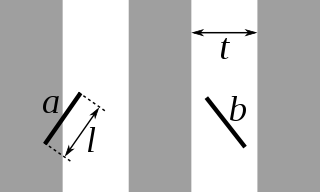
\includegraphics[width=0.4\linewidth]{figure/buffon1.png} 
\caption{The $a$ needle crosses the line, whereas the $b$ needle does not. Source: Wikipedia}
\label{fig:buffon1}
\end{figure}

\section{Derivation}

The problem in more mathematical terms is: Given a needle of length \(a\) dropped on a plane ruled with parallel lines \(d\) units apart, what is the probability that the needle will lie across a line upon landing?
Various sources exist for deriving the desired probability. 
See for example \cite{mantel1953extension} and \cite{duncan1967variation}.

Consider the ``short needle'' case (\(a < d\)). For a randomly thrown needle, let \(\theta\) be the angle that the needle makes between it and the horizontal lines, where \(0\leq \theta \leq \pi/2\). 
Note that the cases when the needle makes a `negative slope', i.e.~\(\theta > \pi/2\) can be ignored because these can be argued to be identical to cases where \(\tilde\theta = (\pi -\theta) \in [0,\pi/2]\) vis-à-vis the intersection of the needle with the horizontal lines.

\begin{figure}[htbp]
\centering 
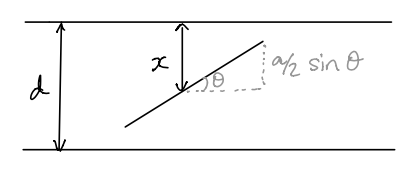
\includegraphics[width=0.5\linewidth]{figure/buffon2} 
\caption{A randomly thrown short needle on a horizontal plane.}
\label{fig:buffon2}
\end{figure}

Let \(x\) be the shortest distance between the centre of the needle and a horizontal line. 
Thus \(0\leq x \leq d/2\). 
Using standard trigonometry, the \textit{vertical half-height of the needle}, as measured between the centre of the needle to the ``top point'' of the needle closest to one of the horizontal lines, is given by \((a/2)\sin\theta\).
\textbf{We realise that the needle crosses any horizontal line if $x < (a/2)\sin\theta$}.

As the needles are thrown randomly on the plane, values of \(\theta\) and of \(x\) are \textit{uniformly random}. 
Also, the values of \(\theta\) and \(x\) do not influence one another, and thus are independent of each other. 
Recall that a random variable \(Y\) distributed as \(\operatorname{Unif}(\alpha,\beta)\) has pdf given by \(f(y) = 1/(\beta-\alpha)\), where \(y\) takes values in \([\alpha,\beta]\).
Therefore, we may write \(\theta \sim \operatorname{Unif}(0,\pi/2)\) with pdf \(f(\theta)=2/\pi\), and \(x \sim \operatorname{Unif}(0,d/2)\) with pdf \(f(x)=2/d\). 
Additionally, the bivariate random variable \(\mathbf z = (\theta,x)\) is also uniformly distributed, with pdf 
\[
f(\mathbf z) = f(\theta,x) = f(\theta)f(x) = \frac{4}{\pi d},
\] 
\(0\leq\theta\leq \pi/2\), \(0\leq x \leq d/2\). 
The probability of crossing (\(p\)) is given by integrating the pdf over the set \(\{(x,\theta) \mid x < (a/2)\sin\theta \}\), i.e. 
\begin{align*}
p &= \iint\limits_{\{x < (a/2)\sin\theta\}} \frac{4}{\pi d} d x d\theta \\
&= \int_{\theta=0}^{\pi/2} \int_{x=0}^{(a/2)\sin\theta} \frac{4}{\pi d} d x d \theta \\
&= \frac{4}{\pi d} \int_{\theta=0}^{\pi/2} (a/2)\sin\theta d \theta \\
&= \frac{2a}{\pi d}
\end{align*}

Alternatively, we can obtain the probability by viewing the problem geometrically. 
Each point represents exactly one realisation of the position of the randomly landed needle. 
The points which represent needles crossing the line are shaded, and these are exactly the points in the set \(\{(x,\theta)| x < (a/2)\sin\theta \}\). 
The area of the shaded region is obtained by integrating the function \(f(y) = (a/2)\sin y\) from \(y=0\) to \(y=\pi/2\), giving us \(a/2\).
Now the total area of the state space is the rectangular area \(\pi/2 \times d/2 = \pi d / 4\). 
Therefore, the probability required is
\begin{equation}
p = \frac{\text{Area of shaded region}}{\text{Total area}} = \frac{2a}{\pi d}.
\end{equation}

\section{Estimating $\pi$}

Suppose that the value of \(p\) is estimated by a suitable value
\(\hat p\). 
Then the value \(\pi\) can then be estimated too by rearranging the equation in \eqref{eq:probres}: 
\begin{equation}
\hat\pi = \frac{2a}{\hat p d}.
\end{equation} 
Then the remaining question is how to obtain an estimate \(\hat p\). 
From a frequentist perspective, one would be tempted to actually throw a bunch of needles and record how many times the needle actually crosses the line. 
Let \(B\) be the total number of times needles were thrown. 
The required estimator would then be 
\[
\hat p = \frac{\text{\# times cross the line}}{B}.
\] 
Indeed, such an estimator would also be guaranteed to converge to the actual true value \(p\) as \(B\to\infty\) by the weak law of large numbers.

It was said that Buffon actually performed this experiment not with needles, but with baguettes thrown from a tower onto the city square below. 
Perhaps slightly less excitingly, we will perform the simulations in R code, and this will be explained in the next section.

\section{Simulations}

There are two determinants of the way the needles are dropped: 
the location of the midpoint of the needle along the \(y\)-axis (call this
\texttt{y}); 
and the angle that the needle makes with the horizontal axis (call this \texttt{angle}). 
Assuming independent and uniform throws of the needle, \texttt{y} can be simulated using \texttt{runif()} with \texttt{min\ =\ -d/2} and \texttt{max\ =\ d/2}, where \texttt{d} is defined to be the distance between two lines. 
This makes it such that the 0 line is in the middle, and the closest distance \(x\) between the needle midpoint and a horizontal line is obtained by \texttt{d/2\ -\ abs(y)}. 
Note that the \texttt{x} position along the horizontal axis is not too important here; 
but for nice results we simulate \texttt{x} uniformly from \texttt{runif(min\ =\ 0,\ max\ =\ 2\ *\ d)}.

The \texttt{angle} may be also be uniformly distributed, and the minimum and maximum value for this variable is 0 and \(\pi\) respectively. 
Depending on the value of \texttt{angle}, the corresponding pair of end points for the randomly thrown needle can be obtained using basic trigonometry, deduced from the midpoint position \texttt{x} and \texttt{y}. 
That is, the upper and lower end-point in the \(y\)-axis direction is \texttt{y\ +\ (a/2)\ *\ sin(angle)} and \texttt{y\ -\ (a/2)\ *\ sin(angle)}, irrespective of the value of \texttt{angle}. 
The left and right end-point in the \(x\) axis direction meanwhile is \texttt{x\ -\ (a/2)\ *\ sin(angle)} and \texttt{x\ +\ (a/2)\ *\ sin(angle)} for when \texttt{angle} is less than \(\pi/2\); if \texttt{angle} is greater than \(\pi/2\) then these values are reversed.

To run the simulation, values of \texttt{a} and \texttt{d} have to be chosen such that \texttt{a} \textless{} \texttt{d}. 
Here, we chose \texttt{a\ \textless{}-\ 3} and \texttt{d\ \textless{}-\ 4}. 
We need to also choose some value \texttt{B}, noting that the bigger this number is, the better the results. 
We chose \texttt{B\ \textless{}-\ 2000}.
Figure \ref{fig:sim2} below plots the first 250 iterations of the needle
simulation. 
The needles have been colour coded according to whether or not the horizontal lines were crossed.

\begin{figure}
\centering 
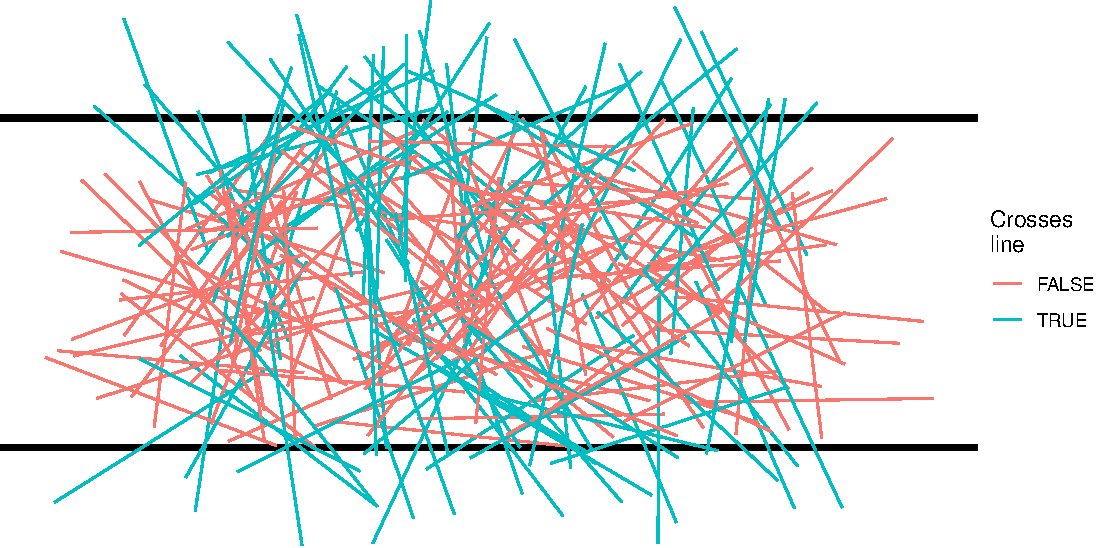
\includegraphics[width=\linewidth]{figure/sim2-1}
\caption{The first 250 random throws of the needles.}
\label{fig:sim2}
\end{figure}

Of course, the main interest is in the estimate \(\hat\pi\). 
The value of \(\hat\pi\) is tracked as the simulation progresses (a running estimate) and plotted against the simulation number. The results are show in Figure \ref{fig:sim3}. 
The value \(\hat\pi\) is seen to get closer to the actual value of \(\pi\) (horizontal dotted line) as the simulation increases. 
After 2000 simulations, the value of \(\pi\) was estimated to be 3.168, giving an absolute error value of 0.026. 
The estimate for first 500 needle tosses seem to be quite poor, suggesting that if this experiment was done in actuality, a really large sample size would be required.

\begin{figure}
\centering 
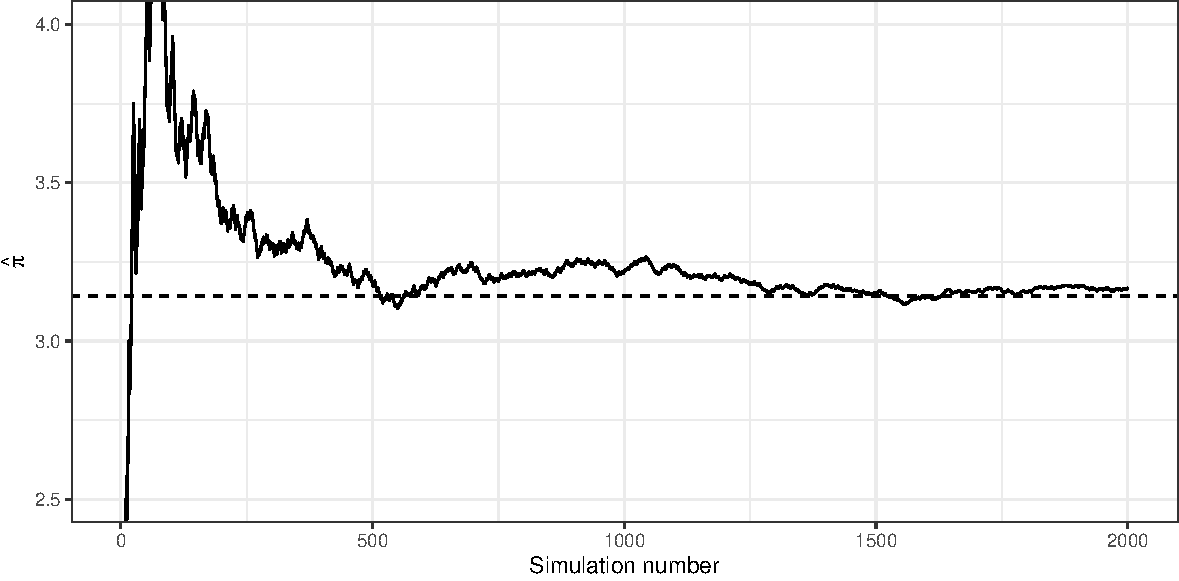
\includegraphics[width=\linewidth]{figure/sim3-1} 
\caption{The running estimate for the value of $\pi$.}
\label{fig:sim3}
\end{figure}

\section{Conclusions}

A computer-based simulation of the Buffon's needle problem was
presented. 
For a simulation size of 2000, the value of \(\pi\) was
estimated to be 3.168, giving an absolute error value of 0.026. 
In the course of conducting this mini project, further questions were pondered:
\begin{enumerate}
\item What values of \(a\) and \(d\) are optimal in terms of minimising the error for predicting \(\pi\)?
\item
  What needs to be changed, if at all, for the ``long needle'' scenario, i.e.~for values \(a > d\)?
\end{enumerate}
Both seemingly interesting questions which are hoped to be tackled another time.

\appendix

\section{Code for simulation}


\begin{verbatim}
set.seed(261022)
B <- 2000  # Number of simulations
d <- 4     # Distance between horizontal lines
a <- 3     # Length of needle

# Create the tibble
plot_df <-
  tibble(
    throw = 1:B,
    x = runif(B, 0, 2 * d),
    y = runif(B, 0 - d/2, d/2),
    angle = runif(B, 0, pi),
    x1 = case_when(
      angle > pi/2 ~ x + a/2 * cos(pi - angle), 
      TRUE ~ x - a/2 * cos(angle)
    ),
    y1 = y - a/2 * sin(angle),
    x2 = case_when(
      angle > pi/2 ~ x - a/2 * cos(pi - angle), 
      TRUE ~ x + a/2 * cos(angle)
    ),
    y2 = y + a/2 * sin(angle),
    s = d/2 - abs(y),  # shortest distance between midpoint and hor. line
    theta = case_when(  # theta value in [0,pi/2]
      angle > pi/2 ~ pi - angle, 
      TRUE ~ angle
    ),
    cross = s < a/2 * sin(theta),  # does the needle cross?
    pi_pred = 2 * a / (cummean(cross) * d)  # running estimate for pi
  )

# Estimate for pi
pihat <- 2 * a / (mean(plot_df$cross) * d)
\end{verbatim}

\section{Code for figures}

\subsection{Needle simulation figure}

\begin{verbatim}
plot_df %>%
  slice_head(n = 200) %>%
  ggplot() +
  geom_hline(yintercept = c(-d/2, d/2), size = 1.5) +
  geom_segment(aes(x1, y1, xend = x2, yend = y2, group = throw, col = cross)) +
  coord_equal() +
  theme_void() +
  labs(col = "Crosses\nline")
\end{verbatim}

\subsection{Running estimate figure}

\begin{verbatim}
ggplot(plot_df, aes(throw, pi_pred)) +
  geom_line() +
  geom_hline(yintercept = pi, linetype = "dashed") +
  theme_bw() +
  coord_cartesian(ylim = c(2.5, 4)) +
  labs(y = expression(hat(pi)), x = "Simulation number")
\end{verbatim}

\printbibliography


\end{document}
